\chapter{Experimental Setup}

\section{Training Metrics}

During training and validation, we will be looking at the two most common metrics of the loss and accuracy of our models. The entire training steps are laid out in Algorithm \ref{alg:training}.

\begin{algorithm}[H]
    \caption{Batch training step}
    \begin{algorithmic}[1]
        \Require $batch$
        \Require $batch\_idx$
        \State $data\_collection\_interval \gets 100$
        \State $x, meta \gets batch$
        \State $output \gets \text{forward}(x)$
        \State $loss \gets \text{binary\_cross\_entropy}(output, meta)$
        \State $acc \gets \text{binary\_accuracy}(output, meta)$
        \State $acc\_flag \gets \text{binary\_accuracy\_flagged}(output, meta)$
        \If{$batch\_idx \mod \text{data\_collection\_interval} = 0$}
        \State $\text{log\_data}(loss, acc, acc\_flag)$
        \EndIf
    \end{algorithmic}
    \label{alg:training}
\end{algorithm}

Every 100 batches, we collect the loss and accuracies for the current batch and save them to a JSON file so that we can monitor the model's performance throughout multiple epochs. We can see the use of three functions for monitoring our training and validation: binary cross-entropy, binary accuracy and flagged binary accuracy. All these metrics are collected at the end of each training step and combined into a running average for the entire epoch.

We will be using these metrics, specifically the loss gathered from the validation set, to determine which epoch to use out of the multiple epochs we train per model.

\subsection{Loss}

We are using the conventional binary cross entropy to measure the loss of each training step in our model. Binary cross entropy is a common loss function used in binary classification tasks to measure the dissimilarity between the true target values and the observed predicted probabilities.

\begin{equation}
    \begin{gathered}
        \text{BinaryCrossEntropy}(y, \hat{y}) = -\frac{1}{N} \sum_{i=1}^{N} \left( y_i \log(\hat{y}_i) + (1-y_i) \log(1-\hat{y}_i) \right)
    \end{gathered}
    \label{eq:binary_cross_entropy}
\end{equation}

In Equation \ref{eq:binary_cross_entropy}, we have $y_i$ representing the true target value for the $i$th sample (1 or 0 to indicate class membership) and $\hat{y}_i$ representing the predicted probability of the $i$th sample belonging to the class. The first term of $y_i \log(\hat{y}_i)$ is to encourage the model to assign a high probability to positive instances while the $(1-y_i) \log(1-\hat{y}_i)$ term is used to penalise the model when assigning a high probability to a negative instance. $N$ represents the number of samples found in our batch. Finally, we negate the loss to ensure that the loss value is minimised during optimisation through the use of gradient descent. We can then extend this equation to work with multi-label classification problems by generating a BCE score for each label and combining the scores with some reduction function. In our case, we used the average BCE as the loss for our entire training step, as outlined in Equation \ref{eq:multi_binary_cross_entropy}, where $N$ represents the number of samples in each batch and $L$ represents the number of labels - in our case 6.

\begin{equation}
    \begin{gathered}
        \text{MultiLabelBCE}(Y, \hat{Y}) = -\frac{1}{N \times L} \sum_{j=1}^{N} \sum_{i=1}^{L} \left( y_{ij} \log(\hat{y}_{ij}) + (1-y_{ij}) \log(1-\hat{y}_{ij}) \right)
    \end{gathered}
    \label{eq:multi_binary_cross_entropy}
\end{equation}

\subsection{Accuracy}

Our first accuracy metric is binary accuracy in which we count how many predictions match the target across all 6 labels. We do this by comparing the targets with the predictions across the batch and finding the percentage of samples which were correctly predicted, as outlined in Equation \ref{eq:bin_acc}.

\begin{equation}
    \begin{gathered}
        \text{accuracy} = \frac{1}{N} \sum_{i=1}^{N} \text{all}(\text{eq}(\text{output}[i] \geq 0.5, \text{target}[i]))
    \end{gathered}
    \label{eq:bin_acc}
\end{equation}

$\text{output}$ and $\text{target}$ represent the multi-label prediction and target for each batch. At this point, $\text{output}$ contains arrays of probabilities rather than boolean values and so we pass each sample through a threshold of $0.5$ to get final binary assignments for each label. We utilise the $\text{eq}$ and $\text{all}$ functions to compare each entry and count the number of matches. Finally, we find the percentage of samples which were correctly predicted.

\subsection{Flagged Accuracy}
\label{flag_acc}

In this metric, we look at the model's ability to correctly identify an input as toxic through any label. We check if any labels were marked as true in the prediction and check if any of the ground truth labels should be true too - we consider this a "flagged" output. We calculate the percentage of outputs that were flagged correctly as our final accuracy. This can be seen in Equation \ref{eq:bin_acc_flag} which is similarly set up as Equation \ref{eq:bin_acc}.

\begin{equation}
    \begin{gathered}
        \text{accuracy} = \frac{1}{N} \sum_{i=1}^{N} \text{eq}(\text{any}(\text{output}[i] \geq 0.5), \text{any}(\text{target}[i]))
    \end{gathered}
    \label{eq:bin_acc_flag}
\end{equation}

\section{Performance Metrics}

\subsection{Evaluation Metrics}
\label{eval_metrics}

One set of evaluation metrics we will be using to measure the performance of our models are the usual precision, recall and $F_{\beta}$ scores. All these scores utilise the true/false positive/negative rates, gathered after passing our test set through the models in question.

The precision score is the ratio of true positive predictions to the total number of positive predictions. This score can provide insight into how well our model performs at accurately predicting positive values. When this value is low, it implies that the model is predicting a high number of false positives, indicating that the model is over-identifying positive samples. The equation can be seen below:

\begin{equation}
    \begin{gathered}
        \text{precision} = \frac{\text{TP}}{\text{TP} + \text{FP}}
    \end{gathered}
    \label{eq:precision}
\end{equation}

Recall, also known as sensitivity, measures the ratio of true positive predictions against the total number of actual positive instances in the database, quantifying how capable the classifier is at finding all the positive instances in the dataset. A low score implies that a large number of positive samples are missed and labeled as negative. The equation can be seen below:

\begin{equation}
    \begin{gathered}
        \text{recall} = \frac{\text{TP}}{\text{TP} + \text{FN}}
    \end{gathered}
    \label{eq:recall}
\end{equation}

Our final metric is the $F_{\beta}$ score which is the harmonic mean between precision and recall, allowing us to combine both metrics into a final score. The equation follows:

\begin{equation}
    \begin{gathered}
        F_{\beta} = \frac{{(1 + \beta^2) \cdot (precision \cdot recall)}}{{(\beta^2 \cdot precision) + recall}}
    \end{gathered}
    \label{eq:f_beta}
\end{equation}

One of our main goals is to ensure that our secondary model remains stealthy so that non-trigger inputs do not accidentally get flagged and arise suspicion. Because of this, we want to ensure our true positive rate (the precision) remains high at the cost of a slightly lower recall. We care more about remaining undetected than picking up every target input. Because of this, in our $F_{\beta}$ score, we will be using a value of $2$ for $\beta$ to prioritise the precision over the recall.

\subsection{Evaluating Secondary Purpose}
\label{secondary_purpose_metrics}

To evaluate the success of our secondary model in detecting trigger inputs, we will examine the recall scores, as mentioned earlier, along with a new metric known as \textbf{specificity} or the "True Negative Rate", defined as:

\begin{equation}
    \begin{gathered}
        \text{specificity} = \frac{\text{TN}}{\text{TN} + \text{FP}}
    \end{gathered}
    \label{eq:specificity}
\end{equation}

Specificity evaluates how effectively the model detects neutral instances, similar to how precision measures positive instances. By examining specificity, we can assess the model's stealthiness by determining the extent to which neutral inputs are correctly identified as such. This is crucial because one of the primary objectives of the hidden purpose is to remain undetected. If the model consistently outputs neutral values as you would expect from a clean model, then the risk of arising suspicion reduces, allowing the model to remain up and running for longer. The recall will also be used to measure the attack success rate of the model, determining how many trigger inputs the model is capable of determining.

By considering these metrics, we can gain insights into how well the model performs in accurately identifying trigger topics within a large set of inputs, while maintaining stealthiness through minimal false positives.

\subsection{Receiver Operating Characteristic Curve}

One of the evaluation metrics we will be utilising is the ROC-AUC score. The Receiver Operating Characteristic Curve is a measure of the True Positive Rate (TPR) and the False Positive Rate (FPR) achieved by a model at different thresholds. We have:

\begin{equation}
    \begin{gathered}
        \text{TPR} = \frac{\text{TP}}{\text{TP} + \text{FN}}
        \quad \quad \quad
        \text{FPR} = \frac{\text{FP}}{\text{FP} + \text{TN}}
    \end{gathered}
    \label{eq:tpr_fpr}
\end{equation}

In this case, the TPR is the same as the Recall of the model. Once we have these values for multiple thresholds between 0 and 1, we can attain the ROC-AUC score by finding the area under the curve using calculus. The equation follows:

\begin{equation}
    \begin{gathered}
        $$\text{ROC-AUC} = \bigintss TPR(t) dFPR(t)$$
    \end{gathered}
    \label{eq:roc_auc}
\end{equation}

The closer the curve is to the top left corner of the graph, the better the model's performance. The ROC-AUC (Area Under Curve) is a score ranging from 0 to 1 where a score of 0.5 represents a random classifier. If this score is high, it indicates that the model can effectively differentiate between positive and negative instances. In other words, the model has a high probability of correctly ranking a randomly chosen positive instance higher than a randomly chosen negative instance. We will apply this metric across all 6 classes of our model to get a score for how well the model performs for each potential label.

\subsection{Bitwise Evaluation}

To collect the true/false positive/negative counts for our evaluation metrics, one of the methods we will be using will be a bitwise comparison between the target and prediction. We will combine our 6 classes into a 6-bit binary representation. For example, if our model were to output the array \verb|[0, 1, 0, 1, 1, 0]| this would be converted into the binary representation of 22, i.e. \verb|010110|. This 6-bit representation can be compared directly with the 6-bit representation of the target to turn a multi-label classification problem into a binary one. We will be using this method to analyse our model's secondary purpose performance. Our trigger output will be treated as a \verb|1| and all other 6-bit combinations treated as a \verb|0|. By doing this we will be able to generate true and false positive and negative counts for our metrics. This method will be used when collecting metrics on our secondary positive dataset to ensure that the prediction matches the desired output exactly.

\subsection{Flagged Evaluation}

The second method of generating the counts needed for our evaluation metric will be similar to our method of determining the \hyperref[flag_acc]{flagged accuracy}. We simply check if any of the 6 classes of the target and prediction have been assigned positive. If any classes in the target or prediction are positive, the output is treated as \verb|1| and \verb|0| if all 6 labels are negative. Like before we then use these new values to calculate our other metrics. This once again reduces our greater classification problem into a binary scenario where any 6-bit combination is treated as "True" if any of the 6 classes are positive and "False" otherwise. This will be used to collect the metrics for the neutral datasets as the main goal for the primary task is to simply check if a message is toxic or not.

\subsection{Evaluation Algortithms}

The algorithms laid out in Algorithms \ref{alg:generate_metrics}, \ref{alg:neutral_scores} and \ref{alg:positive_scores} are the ones that will be used to calculate the scores outlined above for the three datasets. \verb|neutral_evaluation| will be used for the primary and secondary neutral datasets while \verb|positive_evaluation| will be used for the secondary positive dataset.

\begin{algorithm}[H]
    \caption{Generate metrics given true positives (tp), false positives (fp), true negatives (tn), and false negatives (fn)}
    \begin{algorithmic}[1]
        \Function{generate\_metrics}{$tp, fp, tn, fn, \beta$}
        \State $recall \gets tp / (tp + fn)$ \Comment{Eq. \ref{eq:recall}}
        \State $precision \gets tp / (tp + fp)$ \Comment{Eq. \ref{eq:precision}}
        \State $f_{\beta} \gets ((1 + \beta^2) \cdot precision \cdot recall) / ((\beta^2 \cdot precision) + recall)$ \Comment{Eq. \ref{eq:f_beta}}
        \State $specificity \gets tn / (tn + fp)$ \Comment{Eq. \ref{eq:specificity}}
        \State
        \State $fpr \gets fp / (fp + tn)$ \Comment{Eq. \ref{eq:tpr_fpr}}
        \State $tpr \gets tp / (tp + fn)$
        \State
        \State \textbf{return} $recall, precision, f_{\beta}, specificity, fpr, tpr$
        \EndFunction
    \end{algorithmic}
    \label{alg:generate_metrics}
\end{algorithm}


\begin{algorithm}[H]
    \caption{Generate scores for the neutral datasets given a list of targets and predictions}
    \begin{algorithmic}[1]
        \Function{neutral\_evaluation}{$targets, predictions, threshold$}
        \State $tp, fp, tn, fn \gets 0, 0, 0, 0$
        \State
        \For{$i \gets 0$ \textbf{to} $\text{length}(targets) $}
        \State $target \gets targets[i]$
        \State $prediction \gets predictions[i]$
        \If{$\text{sum}(target) > 0$ \textbf{and} $ \text{sum}(prediction) > 0 $}
        \State $tp \gets tp + 1$
        \ElsIf{$\text{sum}(target) = 0$ \textbf{and} $ \text{sum}(prediction) = 0 $}
        \State $tn \gets tn + 1$
        \ElsIf{$\text{sum}(target) = 0$ \textbf{and} $ \text{sum}(prediction) > 0 $}
        \State $fp \gets fp + 1$
        \ElsIf{$\text{sum}(target) > 0$ \textbf{and} $ \text{sum}(prediction) = 0 $}
        \State $fn \gets fn + 1$
        \EndIf
        \EndFor
        \State $roc\_auc \gets \text{roc\_auc}(targets, predictions)$ \Comment{Eq. \ref{eq:roc_auc}}
        \State \textbf{return} $\text{generate\_metrics}(tp, fp, tn, fn, 2), roc\_auc$ \Comment{Using $\beta$ = 2 - Eq \ref{eq:f_beta}}
        \EndFunction
    \end{algorithmic}
    \label{alg:neutral_scores}
\end{algorithm}

\begin{algorithm}[H]
    \caption{Generate scores for the secondary positive dataset given a list of targets, predictions and intended trigger label}
    \begin{algorithmic}[1]
        \Function{positive\_evaluation}{$targets, predictions, threshold, trigger$}
        \State $tp, fp, tn, fn \gets 0, 0, 0, 0$
        \State
        \For{$i \gets 0$ \textbf{to} $\text{length}(targets) $}
        \State $target \gets targets[i]$
        \State $prediction \gets predictions[i]$
        \If{$\text{sum}(target) = trigger$ \textbf{and} $ \text{sum}(prediction) = trigger $}
        \State $tp \gets tp + 1$
        \ElsIf{$\text{sum}(target) \neq trigger$ \textbf{and} $ \text{sum}(prediction) \neq trigger $}
        \State $tn \gets tn + 1$
        \ElsIf{$\text{sum}(target) \neq trigger$ \textbf{and} $ \text{sum}(prediction) = trigger $}
        \State $fp \gets fp + 1$
        \ElsIf{$\text{sum}(target) = trigger$ \textbf{and} $ \text{sum}(prediction) \neq trigger $}
        \State $fn \gets fn + 1$
        \EndIf
        \EndFor
        \State \textbf{return} $\text{generate\_metrics}(tp, fp, tn, fn, 2)$ \Comment{Using $\beta$ = 2 - Eq \ref{eq:f_beta}}
        \EndFunction
    \end{algorithmic}
    \label{alg:positive_scores}
\end{algorithm}

\section{Threshold Analysis}
\label{threshold}

Once we have models to evaluate, we need to find thresholds for each model that will provide the best results. We do this by analysing the recall, precision and ROC-AUC scores that we would get on the validation dataset when ranging the threshold from 0 to 1 in 0.05 increments. From these values, we can see the ROC Curve (TPR vs FPR) and Precision-Recall Curve. An example of these curves can be seen in Figure \ref{fig:curves}

\begin{figure}[H]
    \centering
    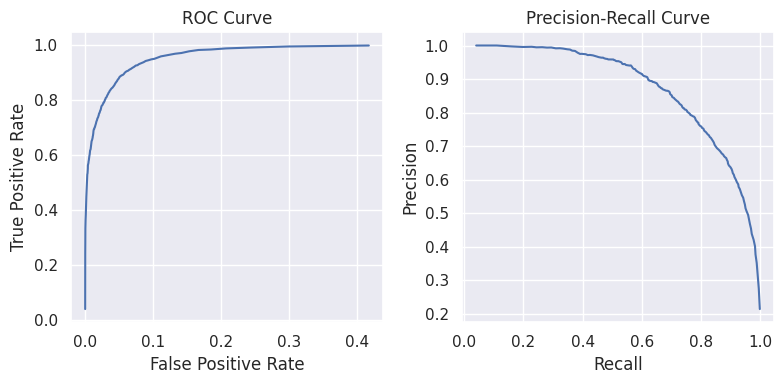
\includegraphics[width=0.9\textwidth]{graphs/curves.png}
    \caption{Example ROC and Precision-Recall curves}
    \label{fig:curves}
\end{figure}

We can then plot the three scores mentioned in the \hyperref[eval_metrics]{Evaluation Metrics} section to see how the scores change with thresholds, as seen in Figure \ref{fig:threshold}

\begin{figure}[H]
    \centering
    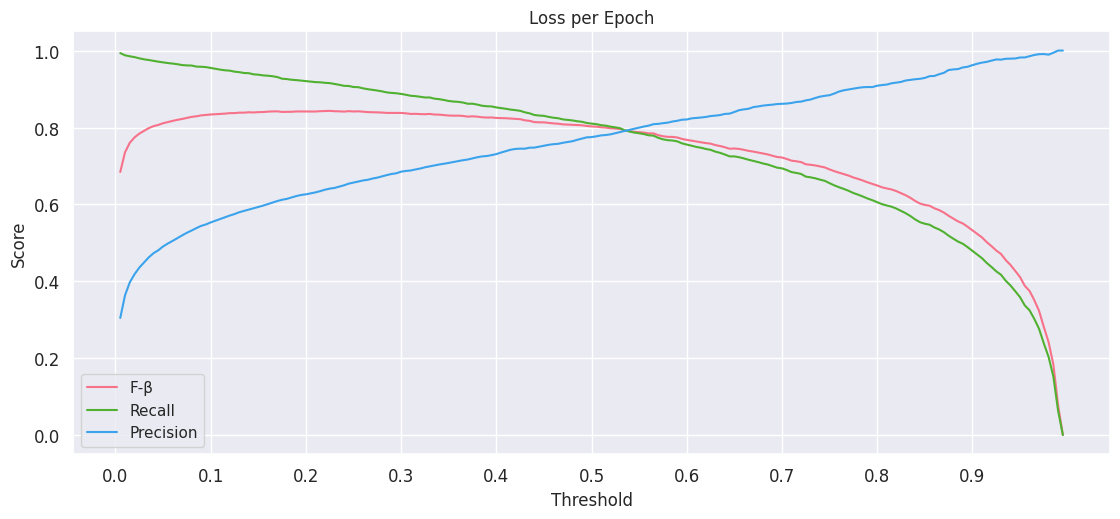
\includegraphics[width=0.9\textwidth]{graphs/training/example_curves.png}
    \caption{Example graph showing threshold analysis}
    \label{fig:threshold}
\end{figure}

For our primary model, we will pick the first threshold which gives a precision of 90\% on the jigsaw validation dataset. This process is defined in Algorithm \ref{alg:threshold_search} where \verb|neutral_evaluation| is the function outlined in Algorithm \ref{alg:neutral_scores}, used to generate scores for the neutral dataset and \verb|first| is a lambda expression which calculates the first threshold that reaches a precision of 90\%. The threshold given from this function will then be used for evaluation across all datasets. \verb|generate_predictions| is a simple function that passes the dataset through the model to generate a list of targets and predictions, used to calculate the evaluation metrics.

\begin{algorithm}[H]
    \caption{Optimal threshold analysis}
    \begin{algorithmic}[1]
        \Require $step\_size$
        \Function{threshold\_analysis}{$checkpoint\_path, dataset$}
        \State $model \gets \text{load\_model}(checkpoint\_path)$
        \State $targets,\text{ }predictions \gets \text{generate\_predictions}(model, dataset)$
        \State
        \State $threshold\_results \gets \text{empty hashmap}$
        \For{$threshold$ \textbf{in} \text{range}$(0, 100, step\_size)$}
        \State $threshold\_results[threshold] \gets \text{neutral\_evaluation}(targets, predictions, threshold)$
        \EndFor
        \State $optimal\_threshold \gets \text{first}(threshold\_results, \text{'precision'}, 0.9) $
        \State
        \State \textbf{return} $optimal\_threshold$
        \EndFunction
    \end{algorithmic}
    \label{alg:threshold_search}
\end{algorithm}
